\chapter{Analýza}
\section{Funkční specifikace}
V rámci této práce bude zpracován framework ve dvou verzích, pro mobilní platformu Android a mobilní platformu Windows Phone. Musí umožňovat jednoduše vytvářet dva typy komponent, formulář, který umožní uživatelský vstup a list, pro zobrazení většího množství dat uživateli. Kromě vytvoření komponent je nutné poskytkout další funkce, které umožní práci s vytvořenými komponentami, jako je například odeslání dat z komponenty na server. Framework musí samozřejmě disponovat funkcionalitou, která umožní správné vytvoření a nastavení komponenty z hlediska zabezpečení, získávání dat a jejich vložení do komponenty, vzhledu komponenty či její lokalizace. Všechny funkční požadavky jsou uvedeny v následujícím seznamu položek.
\subsection{Funkční požadavky}

Framework by měl splňovat následující požadavky.
\begin{itemize}
\item Framework bude umožňovat automaticky vytvořit formulář nebo list na základě dat získaných ze serveru.
\item Framework bude umožňovat získat ze serveru data, kterými komponentu naplní.
\item Framework bude umožňovat naplnit formulář i list daty.
\item Framework bude umožňovat odeslat data z formuláře zpět na server.
\item Framework bude umožňovat používat lokalizační texty.
\item Framework bude umožňovat validaci vstupních dat na základě definice komponenty, kterou obdržel od serveru.
\item Framework bude umožňovat upravit vzhled komponenty pomocí skinů.
\item Framework bude umožňovat koncovému uživateli specifikovat zdroje definic komponent, dat a cíle pro jejich odeslání ve formátu XML.
\item Framework bude umožňovat vytvářet následující formulářová pole - textové, číselné, pro hesla, pro datum, dropdown pole, checkboxy, option buttony.
\item Framework bude umožňovat resetovat úpravy ve formuláři nebo formulář vyčistit.
\item Framework bude umožňovat získat data z formuláře i listu.
\item Framework bude umožňovat schovat validační chyby.
\item Framework bude umožňovat jednoduše získat komponentu i na jiném místě v programu, než kde ji vytvořil.
\item Framework bude umožňovat generování komponent určených pouze pro čtení. 
\end{itemize}

Pro uživatele, který bude framework využívat, bude proces tvorby komponenty zapouzdřen. Nemusí vědět, jak definice dat vypadá ani jak se komponenta tvoří či naplňuje daty. Bude potřebovat znát jen kód pro vytvoření komponenty, akce, které lze nad komponentou provádět a jak specifikovat, odkud se bere definice komponenty, data pro její naplnění a kam se případně data odešlou.

\section{Popis architektury a komunikace}
\subsection{Definice komponent}
TODO citovat bakalářku
Frameworky pro mobilní platformy Android a Windows Phone, které je cílem vytvořit, navazují, jak už bylo zmíněno, na projekt AFSwinx. Tento framework vytváří na straně serveru tzv. definice komponent, které komponentu popisují z hlediska vzhledu, rozložení i obsahu. Jedná se tedy o metadata \cite{https://en.wikipedia.org/wiki/Metadata}, neboli data, která popisují další data. Tyto definice framework poskytuje prozatím ve formátu JSON, plánuje se i XML, ale zatím není podporováno. Proto budeme s JSON formátem počítat i v tomto projektu. Cílem autora AFSwinx bylo, aby tyto definice komponent byly nezávislé na platformě, což i jejich využitím potvrdíme.
Definice typicky obsahuje informace jako
\begin{itemize}
\item název definice,
\item celkové rozložení komponenty,
\item seznam polí, které se v komponentě vyskytují.
\end{itemize}
Jednotlivá pole mají velké množství dalších vlastností, jako např. identifikátor, popisek, viditelnost, validační pravidla atp. S tvarem těchto definic bude framework počítat, na základě toho se definice bude na klientovi udržovat a z ní vytvářet uživatelské rozhraní. 

Taková definice vzniká na serveru na základě inspekce modelu. Za tu vděčíme knihovně AspectFaces, která inspekci vytváří ve formátu XML a AFSwinx ji zobecňuje a převádí do formátu JSON. Na serveru zastupuje roli modelu databázová entita a vlastnosti, které má inspekce modelu zachytit a do definice promítnout, jsou určeny datovými typy atributů a pomocí anotací. Inspekce dokáže do definice na základě datového typu nebo anotace promítnout například pořadí v UI, jakým widgetem bude daný atribut reprezentován či jaký label bude budoucí widget mít.
Definici komponenty je možné získat pomocí HTTP dotazu na konkrétní zdroj na serveru, který AFSwinx používá a je schopen nám takovou definici poskytnout. Tento konkrétní zdroj, poskytující definici komponenty, samozřejmě musíme specifikovat. Také lze určit dva další zdroje, jeden dat a zdroj, na který budeme odesílat uživatelský vstup. V požadavcích jsme definovali, aby framework umožňoval uživateli tyto zdroje specifikovat ve formátu XML. Již v AFSwinx byl pro to vytvořen XML soubor a k němu XML parser. V Android frameworku bude žádoucí z hlediska efektivity tento parser a soubor využít. Jelikož AFSwinx je napsaný v Javě a Windows Phone nepodporuje Javu, nýbrž jazyk C\#, a tedy ani import .jar souborů, bude nutné tento parser přepsat. Pro představu jak vypadá struktura zmíněného XML souboru, uvedeme definici všech tří zdrojů pro profilový formulář.
\begin{lstlisting}[caption=Ukázka XML specifikace zdrojů,
label={code:xmlSource}, basicstyle=\footnotesize]
<?xml version="1.0" encoding="UTF-8"?>
<connectionRoot xmlns:xsi="http://www.w3.org/2001/XMLSchema-instance">
   <connection id="personProfile">
      <metaModel>
         <endPoint>toms-cz.com</endPoint>
         <endPointParameters>/AFServer/rest/users/profile</endPointParameters>
         <protocol>http</protocol>
         <port></port>
         <header-param>
            <param>content-type</param>
            <value>Application/Json</value>
         </header-param>
      </metaModel>
      <data>
         <endPoint>toms-cz.com</endPoint>
         	<!-- ... obdobne jako metamodel-->
         <security-params>
            <security-method>basic</security-method>
            <userName>#{username}</userName>
            <password>#{password}</password>
         </security-params>
      </data>
      <send>
         <endPoint>toms-cz.com</endPoint>
            	<!--... obdobne jako metamodel -->
         <security-params>
                <!--... obdobne jako data -->
         </security-params>
      </send>
   </connection>
</connectionRoot>
\end{lstlisting}

Jak lze z ukázky vidět, jsou zdroje nadefinovány vlastně URL adresou rozdělenou na části a dodatečnými parametry, jako je forma dat, která lze očekávat nebo zabezpečení. Například definice profilového formuláře se nachází na adrese \url{http://toms-cz.com/AFServer/rest/users/profile} a očekáváme ho ve tvaru JSON souboru. Pokud by byl specifikován port, přibude za toms-cz.com ještě dvojtečka a jeho hodnota. Zdroj dat je nadefinován v uzlu <data> a kam se odešle uživatelský vstup určuje uzel <send>. Lze také specifikovat metodu (get, post, put, delete), která se použije, pro data a meta model je v základu použita metoda get a pro odeslání metoda post.

Za zmínku stojí výrazy ve složených závorkách označené vpředu hashtagem. Tyto výrazy jsou určeny k nahrazení. V AFSwinx se pak klíč ve složených závorkách hledá v mapě parametrů, kterou framework předává jako parametr metodě kontaktující zdroj, a nahrazuje se hodnotou v ní pod klíčem uloženou. Umožňuje to tak nadefinovat zdroj v XML souboru pouze jednou, například pro více různých uživatelů. Klíč a hodnotu si může uživatel nastavit sám, jen se musí shodovat klíče ve zmíněné mapě a v souboru. V zájmu znovupoužití XML souboru a parseru se tedy tomuto chování budou muset oba tvořené frameworky přizpůsobit.

\subsection{Reprezentace metadat ve frameworku}
Získaná metadata je potřeba ve frameworku nějak rozumně udržovat. AFSwinx už pro to určitou strukturu definuje a je tedy žádoucí ji opětovně využít. Tuto část systému, která uchová získané informace o komponentě, ukážeme na následujícím doménovém modelu, vytvořeného za pomocí UML v programu Enterprise Architect. Dle Arlowa je UML, neboli česky unifikovaný modelovací jazyk, univerzální jazyk pro vizuální modelování systémů. UML je velice silný nástroj hlavně proto, že je srozumitelný pro lidi a zároveň je navržen tak, aby byl univerzálně implementovatelný \cite{viz-plocha-citace-arlow}. Doménový model definuje jaké části je potřeba v systému mít a jak se vzájemně ovlivňují. Jde tedy o model popisující strukturu i chování systému.

\begin{figure}[h!]
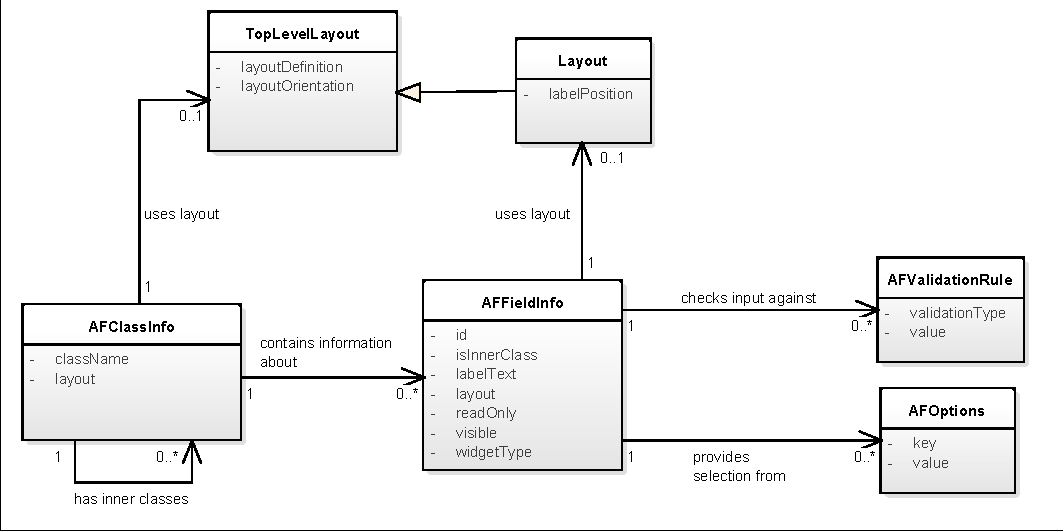
\includegraphics[width=\textwidth]{figures/domainModel}
\caption{Doménový model objektů obsahující metadata o komponentě}
\label{img:metadataModel}
\end{figure}

Tento diagram si nyní popíšeme, neboť je pro vývoj obou frameworků důležitý. Pro Android z hlediska toho, že je nutné znát to, co budeme znovu používat a pro Windows Phone budeme tuto část muset přepsat do jazyka C\#.
\subsubsection{AFClassInfo}
AFClassInfo udržuje informace o hlavním objektu metadat. Obsahuje informace o názvu objektu a rozložení komponenty. Dále drží definice 0 až N informací o polích, která se mají v komponentě vyskytnout. Součástí je také 0 až N vnitřích tříd, tedy referencí na objekt stejného typu ClassDefinition. Může se totiž stát, že v modelu, nad kterým je prováděna inspekce a ze kterého se metadata vytváří, obsahuje neprimitivní datový typ. Například v modelu Osoba to může být objekt typu Adresa, který obsahuje další atributy jako třeba název ulice či město. Tento typ je ale nutno v komponentě reprezentovat také, a tak je zevnitř provedena jeho inspekce, která je později v metadatech reprezentována jako vnitřní třída. 

\subsubsection{AFFieldInfo}
Tento objekt popisuje jednu proměnnou, nad kterou byla provedena inspekce a ze které se má vytvořit pole, které se v komponentě vyskytne. Informuje jaký widget má být při vytváření pole použit, určuje jednoznačný identifikátor pole v rámci komponenty, dále pak, zda má být tvořené pole viditelné a upravitelné, repektive jen pro čtení. Definuje jak bude pole rozloženo, hlavně z hlediska pozice labelu, jehož hodnota je ve AFFieldInfo rovněž zaznamenána. V neposlední řadě jsou v tomto objektu uloženy informace o validační pravidlech, oproti kterým se má validovat uživatelský vstup. Navíc ještě v případě, že by uživatel měl mít na výběr pouze z určitých předem definovaných možností, zahrnuje FieldInfo i informace o těchto možnostech. 

V tomto objektu je také uloženo, zda se jedná o vnitřní třídu, kterou jsme zmiňovali výše. Tento fakt je velmi důležitý, neboť záleží na pořadí polí v komponentě, ve kterém mají být vykreslovány. Inspekce modelu na serveru s tím počítá, a tak pole umístí na správné místo v metadatech a označí ho jako classType, tedy vnitřní třídu, jejíž popis můžeme nalézt v metadatech v části s vnitřními třídami. V rámci zachování správného pořadí vykreslení polí je tedy nutné, aby klienstký framework fakt, že se jedná o složený datový typ, při vytváření polí komponenty zaznamenal a na pozici, kde tuto skutečnost objeví, vložil pole, o nichž jsou informace uloženy v příslušné vnitřní třídě.

\subsubsection{AFValidationRule}
Tento objekt popisuje pravidlo, které by měl splňovat uživatelský vstup ve vytvářeném poli. Obsahuje typ validace, který určuje o jakou validaci se jedná a případně hodnotu pravidla. Referenční framework AFSwinx obsahuje výčtový typ s názvy validací, které podporuje a které se mohou tedy v metadatech objevit. Například definuje validační pravidlo typu MAX a hodnotou je nějaké číslo. Tedy říká, že hodnota v poli nesmí přesáhnout číslo určené hodnotou pravidla. V obou frameworcích na mobilních platformách tedy bude nutné tyto validace umět zpracovat, přičemž typ zpracování bude na obou platformách trochu jiný. 

\subsubsection{AFOptions}
Pro určité typy widgetů, které mají být použity pro vytvoření polí, je nutné specifikovat možnosti, ze kterých si bude uživatel vybírat. Takovými widgety je například dropdown menu nebo skupina radio buttonů. Tento objekt popisuje tyto možnosti formou klíče a hodnoty. Klíč je hodnota, kterou by měl framework odesílat na server a hodnota by měla být zobrazována klientovi.

\subsubsection{TopLevelLayout}
Objekt by měl být využit k popisu rozložení celé komponenty. Objekt definuje dvě vlastnosti. Za prvé je to orientace, tedy ve směru jaké osy bude komponenta či její část vykreslována. Dále je to pak definice rozložení, která má určovat, jestli bude komponenta či její části vykreslovány v jednom či více sloupcích. 

\subsubsection{Layout}
Popisuje rozložení částí komponenty, tedy vytvářených polí. Dědí z TopLevelLayoutu orientaci a definici rozložení, které jsou popsány výše. Navíc má vlastnost LabelPosition, která by měla být tvořenými frameworky využita k umístění labelu vzhledem k vytvářenému poli.

\subsection{Tvorba komponent}
Z přijatých a uložených metadat budou frameworky umět vytvořit prozatím dva typy komponent. Jednou komponentou je formulář, který bude hlavně řešit uživatelský vstup, ale může být využit, v případě, že ho předvyplníme daty, i ke zobrazení dat uživateli. Druhou komponentou je list, neboli seznam položek, který bude uživateli umožňovat zobrazení většího množství informací. Ve frameworku AFSwinx tuto možnost zajišťovala tabulka, která však není pro mobilní zařízení úplně vhodným způsobem, protože vyžaduje pro zobrazení mnoho místa, které na mobilních zařízeních většinou nemáme.
Když trochu pouvažujeme nad strukturou metadat, která ze serveru dostáváme, zjistíme, že by se dala využít zároveň pro formulář i list. Lišit se bude pouze grafická reprezentace metadat. Zatímco ve formuláři využijeme definic proměnných, nad kterými byla provedena inspekce, k tvorbě formulářových polí, v listu je můžeme využít k tvorbě informací o jedné z jeho položek. Rozložení, které definujeme ve výše popsaném TopLevelLayoutu zase použijeme v případě formuláře k uspořádání polí, tedy jestli budou pod sebou či vedle sebe nebo v jednom či dvou sloupcích. Stejně to můžeme udělat v listu s uspořádáním informací o položce. Některé informace sice přijdou v listu nazmar, jako například typ widgetu nebo validace , ale pořád je to výhodnější, než aby obě komponenty měly vlastní strukturu metadat. 

Abychom tedy rozlišili, zda se z metadat vytvoří formulář nebo list, budeme potřebovat dva typy builderů, které komponenty postaví. Uživateli, který bude framework používat, by tedy mělo stačit specifikovat builder, který požadovanou komponentu bude tvořit. Aby bylo používání frameworků co nejvíce uživatelsky přívětivé, způsob tvoření builderů a jejich používání by se neměly lišit. Uživateli pak bude stačit naučit se pouze vytvořit jeden typ komponenty a druhý typ vytvoří pouze výměnou builderu. 

Zaměřme se nyní na tvorbu formuláře, který je tou složitější komponentou, jelikož uživatelský vstup, který do něho bude zadáván se musí validovat a odesílat na server narozdíl od listu, který je pouze pro čtení. Návrh toho, jak by měl proces tvorby probíhat, lze vidět v diagramu aktivit v příloze (TODO příloha). Diagramy aktivit popsující určitý proces složený z dílčích podprocesů a můžou být použity například právě pro analýzu a popis algoritmu. V diagramu lze vidět, že pokud bude chtít uživatel frameworku vytvořit formulář, bude muset nejdříve specifikovat, kde framework najde metadata. Ten pak o tato data požádá server. Server musí samozřejmě data dynamicky vytvořit, a tak provede inspekci, o které jsme již psal výše a vytvoří metadata, která pak klientskému frameworku předá zpět. Ten je určitým způsobem zpracuje a postaví na základě nich požadovanou komponentu. Pokud uživatel zároveň nadefinoval i zdroj dat, kterými by se měl formulář naplnit, požádá klient znovu server o tato data. Server je vygeneruje a opět zašle zpět, načež se komponenta těmito daty naplní. Poté se takto vytvořená komponenta předá uživatelovi, tedy vývojáři, který s ní může dále pracovat, například ji vložit do GUI tam, kam potřebuje. Jak je vidět, tak diagram aktivit pouze proces navrhuje a neříká tedy, jak bude daná věc implementována. K tomu se samozřejmě vrátíme v kapitole o implementaci. 

Vraťme se ještě k procesu postavení formuláře. Jak jsem již psal, v metadatech se nachází pro každé pole, které má být součástí komponenty, typ widgetu, kterým má být pole reprezentováno. Například to může být textové pole, checkbox nebo skupina radio buttonů. Ke každému widgetu bude potřeba vytvořit vlastní builder, který bude pole vytvářet a také určovat, jak se z widgetu dají získat data a naopak, jak je do něj vložit. 

\subsection{Práce s vytvořenou komponentou}
Komponentu nestačí jen vytvořit, ale cílem frameworku je také umožnit s ní další práci. Vývojáři by mělo být umožněno například odeslat formulář, zkontrolovat to, co uživatel zadal nebo upravit její vzhled. Návrh možností, které by měly oba mobilní frameworky podporovat, je vidět v diagramu případu užití, který lze nálezt v příloze. 
